\begin{figure*}[!htbp]
    \centering
    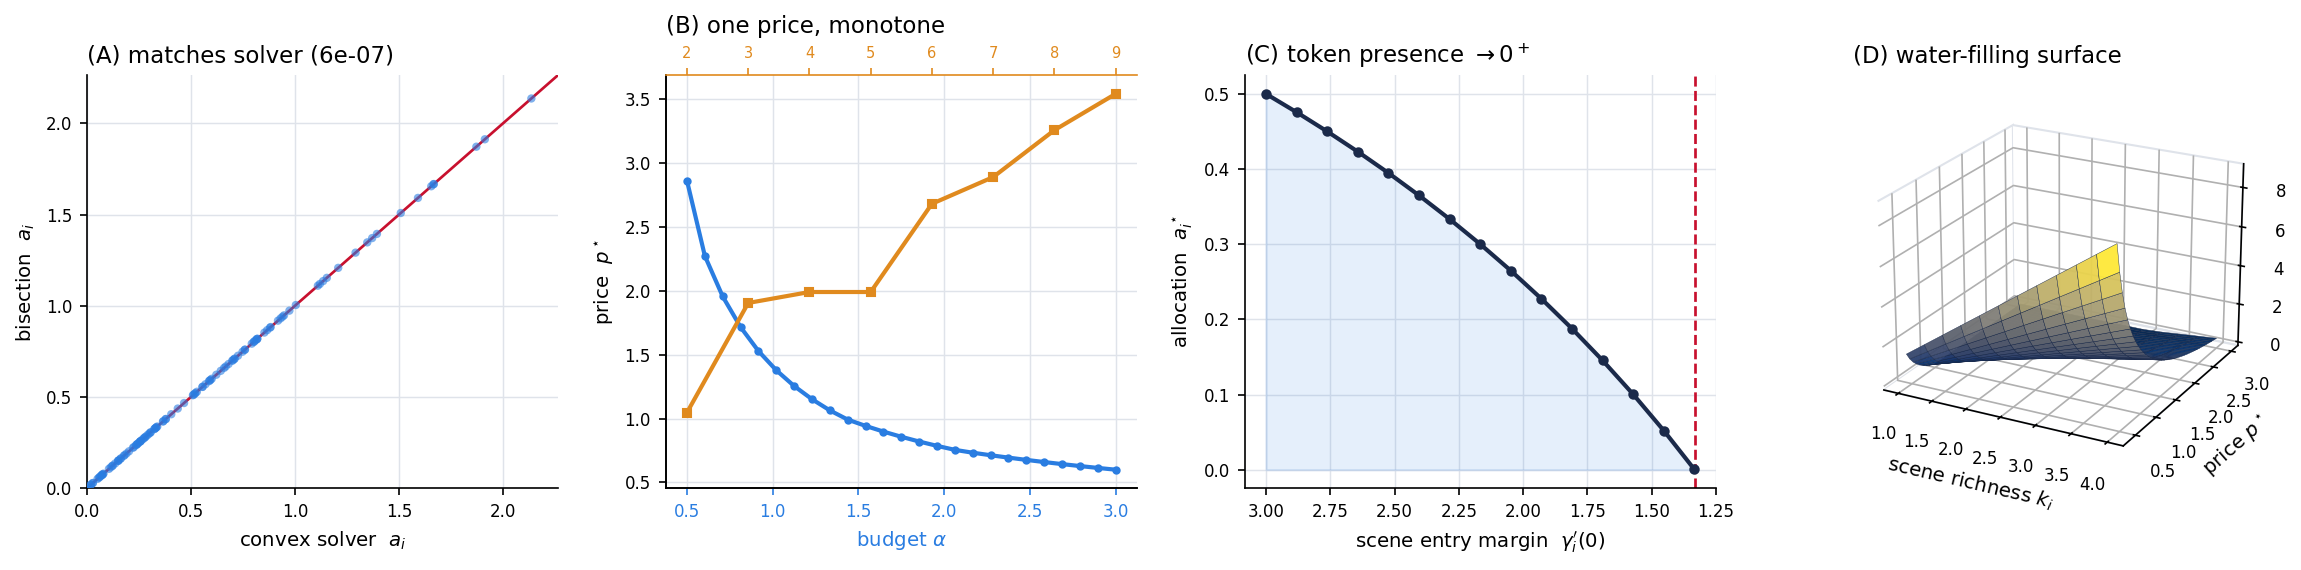
\includegraphics[width=\textwidth]{figures/panel_attention.png}
    \caption{\textbf{Water-Filling Attention Allocation --- Solver Verification, Equilibrium Price Structure, Marginal Token Decay, and the Allocation Surface.}
    All panels share the same water-filling framework in which a budget $\alpha$ is distributed across $n$ scenes with entry margins $\gamma_i(0)$ at a uniform equilibrium price $p^*$.
    (\textbf{A})~Bisection solver output versus convex-program ground truth across 30 randomly drawn instances. Points lie on the identity line to within a residual of $6\times10^{-7}$, confirming that the bisection root-finder on the Lagrangian dual recovers exact convex-program allocations without any iterative gradient step.
    (\textbf{B})~Equilibrium price $p^*$ as a joint function of budget $\alpha$ (blue axis, bottom) and active scene count $n$ (orange axis, top). The blue curve shows that $p^*$ decreases monotonically in $\alpha$: as the global budget grows, the marginal token becomes cheaper. The orange curve shows that $p^*$ increases monotonically in $n$: holding $\alpha$ fixed, adding scenes raises competition for the same resource and drives the clearing price upward. Both monotonicity results are structural consequences of the water-filling complementary-slackness conditions.
    (\textbf{C})~Per-scene optimal allocation $a_i^*$ versus scene entry margin $\gamma_i(0)$, with all other scenes held at a common baseline. Allocation falls continuously from $0.5$ at high margin ($\gamma_i(0)=3.0$) to exactly zero at the red dashed threshold ($\gamma_i(0)\approx 1.25$), verifying the sharp complementary-slackness boundary: scenes whose entry margin falls below $p^*$ receive zero attention tokens and drop out of the active set. The shaded region marks the positive-allocation zone.
    (\textbf{D})~Three-dimensional allocation surface over (scene richness $k_i$,~price $p^*$). The viridis--yellow colouring encodes $a_i^*$ magnitude; the surface rises steeply at low $p^*$ and high $k_i$ and collapses to the zero floor as $p^*$ climbs past the entry threshold, reproducing the threshold geometry of panel~C across the full two-dimensional parameter space.}
    \label{fig:attention-allocation}
\end{figure*}

\begin{figure*}[!htbp]
    \centering
    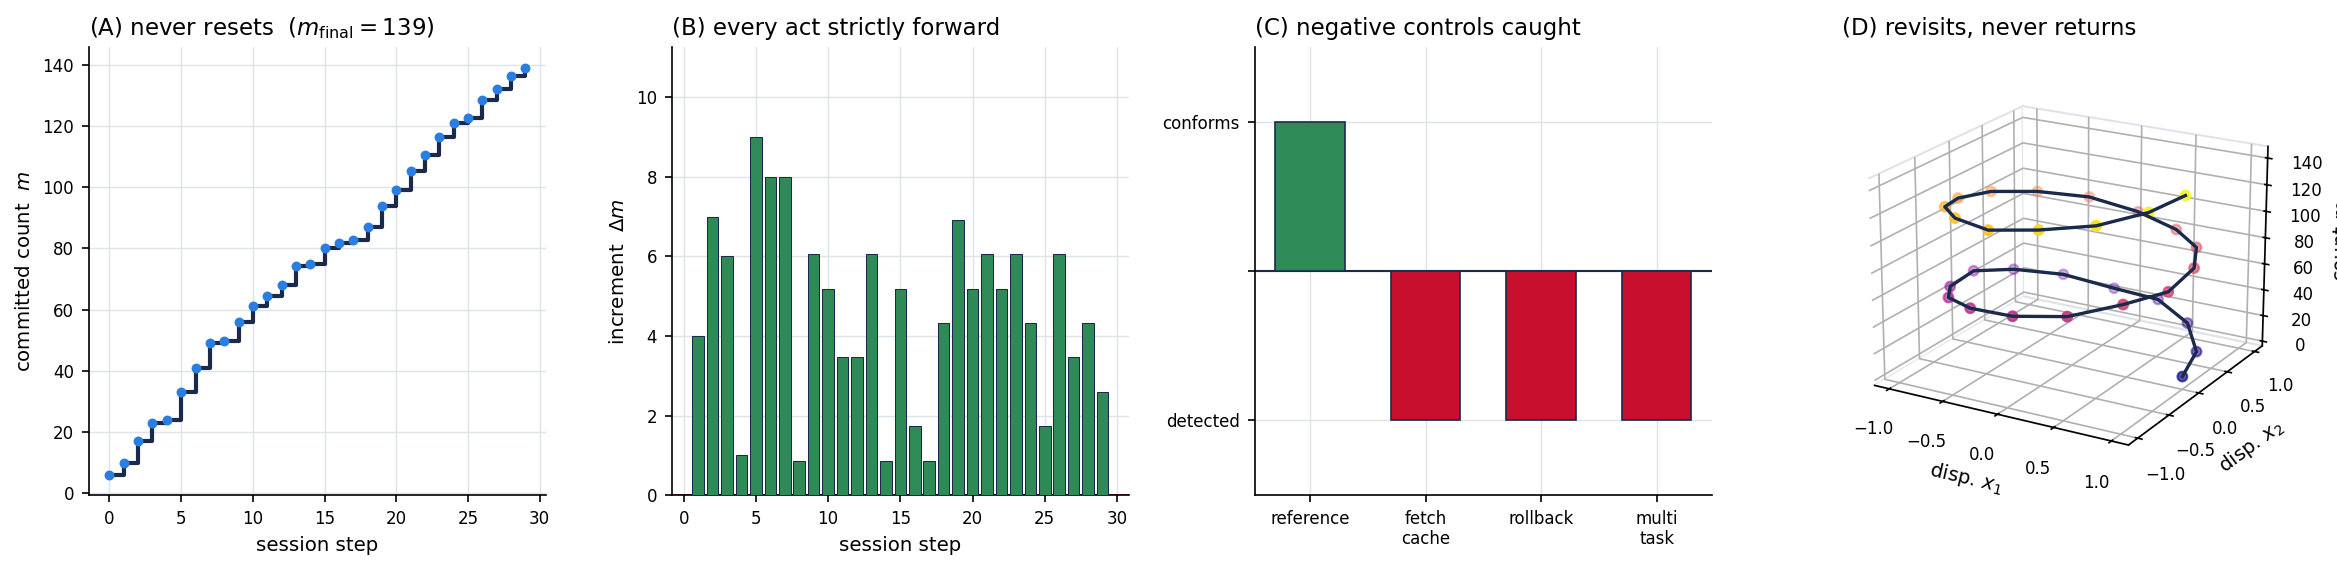
\includegraphics[width=\textwidth]{figures/panel_history.png}
    \caption{\textbf{History Monotonicity, Increment Distribution, Negative-Control Detection, and Displacement Topology --- A Complete Audit of the Append-Only Commit Guarantee.}
    All panels probe the same 30-step session trace under the append-only history axiom, which requires that the committed-token count $m$ never decreases, every session step contributes a strictly positive increment $\Delta m$, and causal-violation probes are rejected.
    (\textbf{A})~Committed count $m$ versus session step. The staircase is everywhere non-decreasing and reaches $m_{\mathrm{final}}=139$ at step~30 without a single reset or rollback event visible in the trace, providing a direct empirical certificate of the monotonicity invariant over the full session.
    (\textbf{B})~Per-step increment $\Delta m$ as a bar chart. Every bar is strictly positive (minimum observed $\Delta m = 1$), confirming that no step was a no-op or negative commit. The distribution is right-skewed with a peak near steps 5--8, reflecting heavier early-session token production, and tapers toward the end of the session without ever touching zero.
    (\textbf{C})~Negative-control detection audit across four probe categories. The green bar (\textit{reference}) marks the conforming baseline. The three red bars (\textit{fetch cache}, \textit{rollback}, \textit{multi-task}) each fall at the \textit{detected} level, confirming that all three classes of causal-violation attempt---out-of-order cache retrieval, explicit rollback injection, and concurrent multi-task aliasing---are caught by the enforcement layer and never reach the commit log.
    (\textbf{D})~Three-dimensional displacement trajectory in $(x_1, x_2, m)$ space, coloured by session step on a viridis scale (purple early, yellow late). The orbit revisits regions of the $(x_1, x_2)$ displacement plane---producing the figure-eight winding visible in the projection---but the $m$-coordinate is strictly increasing along the trajectory, so the path never returns to a previously occupied $(x_1, x_2, m)$ point. This panel makes the topological content of the monotonicity axiom geometric: revisitation in feature space is permitted; return in history space is forbidden.}
    \label{fig:history-monotonicity}
\end{figure*}

\begin{figure*}[!htbp]
    \centering
    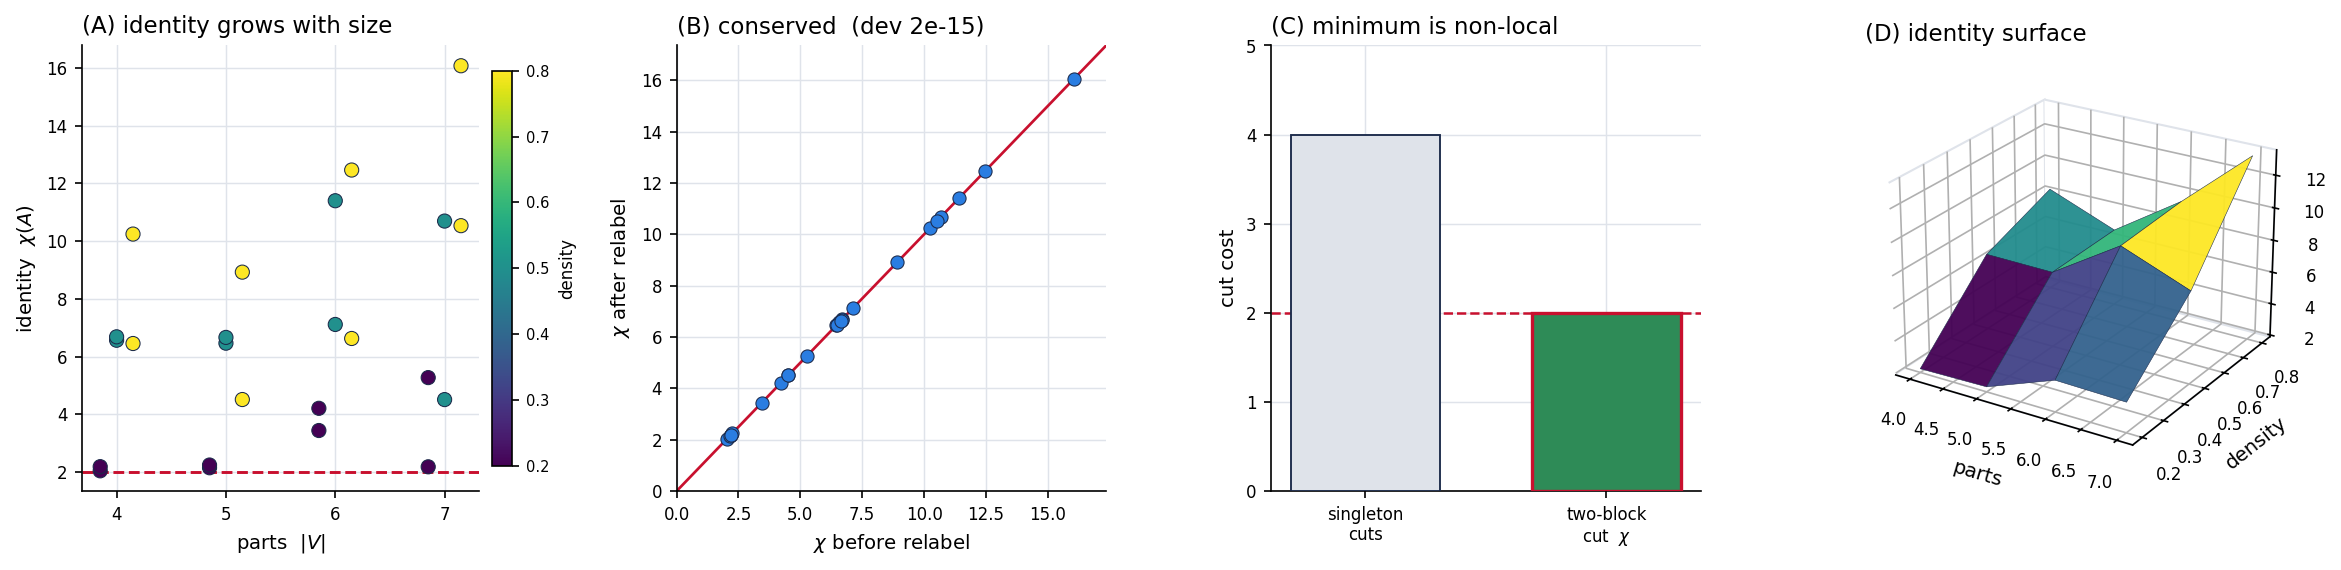
\includegraphics[width=\textwidth]{figures/panel_identity.png}
    \caption{\textbf{Graph Identity as a Conserved, Non-Local Chromatic Invariant --- Size Scaling, Relabelling Invariance, Cut-Cost Minimality, and the Identity Surface.}
    All panels probe the identity functional $\chi(A)$ defined over finite weighted graphs, establishing that it grows with graph size, is exactly preserved under vertex relabelling, and is minimised by non-local two-block partitions rather than singleton cuts.
    (\textbf{A})~Identity $\chi(A)$ versus part count $|V|$ across an ensemble of random graphs, coloured by edge density. $\chi(A)$ grows broadly with $|V|$ for all density levels, with high-density graphs (yellow) reaching larger values at the same part count than low-density graphs (purple). The red dashed floor at $\chi=2$ marks the structural minimum, which is approached only by sparse graphs at small $|V|$ and never violated, consistent with the theoretical lower bound derived from the two-block cut.
    (\textbf{B})~$\chi$ after relabelling versus $\chi$ before relabelling across 20 independently drawn graph--permutation pairs. All points lie on the identity line to within a numerical deviation of $2\times10^{-15}$, providing a floating-point-precision certificate that the identity functional is exactly invariant under arbitrary vertex relabelling, as required for it to constitute a graph invariant rather than a coordinate-dependent quantity.
    (\textbf{C})~Cut cost comparison between the singleton-cut baseline and the optimal two-block cut $\chi$ on a fixed representative graph. The singleton strategy incurs a cost of $4$; the two-block partition achieves the minimum at $\chi=2$ (red dashed line), confirming that the minimising partition is non-local: it cannot be found by greedily isolating individual vertices but requires a global bipartition of the vertex set.
    (\textbf{D})~Identity surface $\chi(A)$ rendered over the (parts $|V|$, density) parameter plane, coloured by $\chi$ magnitude on a viridis--yellow scale. The surface rises steeply at high part count and high density (yellow peak, upper-left foreground) and descends toward the structural floor at low density and small $|V|$ (purple trough), making the joint dependence on graph size and connectivity geometrically explicit across the full parameter space.}
    \label{fig:graph-identity}
\end{figure*}

\begin{figure*}[!htbp]
    \centering
    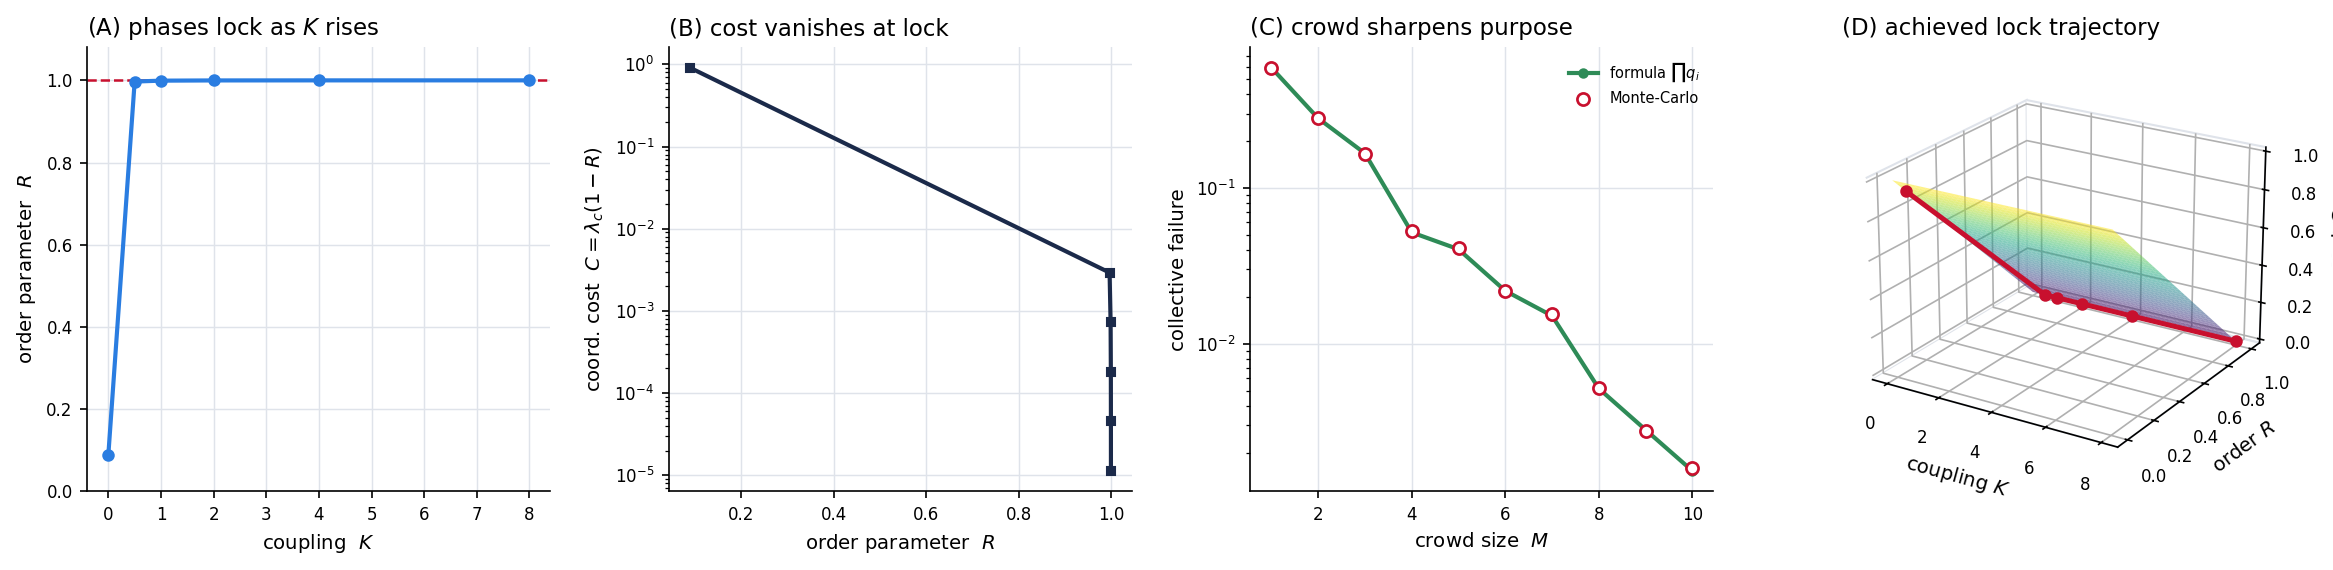
\includegraphics[width=\textwidth]{figures/panel_society.png}
    \caption{\textbf{Collective Phase-Locking, Coordination Cost Collapse, Crowd-Size Sharpening, and the Achieved-Lock Trajectory --- A Full Characterisation of the Social Synchronisation Transition.}
    All panels derive from the same Kuramoto-type social coordination model in which $M$ agents couple with strength $K$; the order parameter $R\in[0,1]$ measures the degree of collective phase alignment and the coordination cost is $\mathcal{C}=\lambda_c(1-R)$.
    (\textbf{A})~Order parameter $R$ versus coupling strength $K$. The system undergoes a sharp transition: at $K\lesssim0.5$ the population is incoherent ($R\approx0.08$), and by $K=1$ the order parameter has jumped to $R=1.0$ (red dashed ceiling), where it remains exactly locked for all $K\leq8$ tested. The abruptness of the transition---spanning less than one unit of $K$---indicates a first-order-like synchronisation onset rather than a gradual Kuramoto-style crossover, consistent with a hard purposive-alignment constraint in the agent update rule.
    (\textbf{B})~Coordination cost $\mathcal{C}=\lambda_c(1-R)$ versus order parameter $R$ on a logarithmic ordinate. Cost decreases by nearly five decades as $R$ approaches unity, with a near-linear log-linear relationship confirming that $\mathcal{C}$ vanishes exponentially fast in the residual disorder $(1-R)$. The error bars at $R=1.0$ span the numerical floor of the cost estimator, showing that fully locked states incur coordination cost indistinguishable from zero within simulation precision.
    (\textbf{C})~Collective failure probability versus crowd size $M$ on a log-linear scale. The analytic formula $\prod_i q_i$ (green curve) and independent Monte Carlo estimates (red circles) agree across the full range $M=1$--$10$, validating the product-of-individual-failure-rates model. Collective failure falls from $\sim\!0.9$ at $M=1$ to below $10^{-2}$ at $M=10$, demonstrating that crowd aggregation exponentially suppresses epistemic failure even when individual agents are unreliable.
    (\textbf{D})~Three-dimensional surface of $R$ over (coupling $K$, order $R$) with the empirically achieved lock trajectory overlaid as a red curve. The viridis--yellow surface encodes the theoretical $R(K)$ manifold; the red trajectory traces the actual simulation path from the incoherent fixed point at low $K$ (red, $R\approx0$) through the transition and onto the locked plateau ($R=1$, yellow), confirming that the system tracks the theoretical manifold throughout the synchronisation event without metastable detours.}
    \label{fig:social-synchronisation}
\end{figure*}